\documentclass[%
%preprint,
 reprint,
superscriptaddress,
%groupedaddress,
%unsortedaddress,
%runinaddress,
%frontmatterverbose,
showpacs,preprintnumbers,
%nofootinbib,
%nobibnotes,
%bibnotes,
 amsmath,amssymb,
 aps,
 prl,
%pra,
%prb,
%rmp,
%prstab,
%prstper,
%floatfix,
]{revtex4-1}

\usepackage{graphicx}% Include figure files
\usepackage{dcolumn}% Align table columns on decimal point
\usepackage{bm}% bold math
%\usepackage{hyperref}% add hypertext capabilities
%\usepackage[mathlines]{lineno}% Enable numbering of text and display math
%\linenumbers\relax % Commence numbering lines

%\usepackage[showframe,%Uncomment any one of the following lines to test
%%scale=0.7, marginratio={1:1, 2:3}, ignoreall,% default settings
%%text={7in,10in},centering,
%%margin=1.5in,
%%total={6.5in,8.75in}, top=1.2in, left=0.9in, includefoot,
%%height=10in,a5paper,hmargin={3cm,0.8in},
%]{geometry}

\begin{document}

%\preprint{APS/123-QED}

\title{Heterogeneity in Nucleosome Spacing Governs Chromatin Elasticity}% Force line breaks with \\
\thanks{A footnote to the article title}%

\author{Bruno Beltran}
\thanks{These authors contributed equally to this work.}%
\affiliation{%
    Biophysics Program, Stanford University, Stanford, California 94305, USA
}%
\author{Deepti Kannan}%
\thanks{These authors contributed equally to this work.}%
\author{Quinn MacPherson}%
\affiliation{%
    Department of Physics, Stanford University, Stanford, California 94305, USA
}%
\author{Andrew J. Spakowitz}%
\email{ajspakow@stanford.edu}%
% \homepage{http://web.stanford.edu/~ajspakow/}%
\affiliation{%
    Chemical Engineering Department, Stanford University, Stanford, California 94305, USA
}%
% \altaffiliation[Also at ]{%
%     Department of Chemical Engineering, Stanford University, Stanford, California 94305, USA
% }%
\date{\today}% It is always \today, today,
             %  but any date may be explicitly specified

\begin{abstract}

%Start with a sentence leading into heterogeneity of proteins binding to DNA.
We propose a coarse-grained model for the effects of nucleosome packaging on the
    physical organization of chromosomal DNA, and present the analytical
    solution in the form of a Green's function.
Our analytical model combines a wormlike-chain treatment of the linker DNA
    connecting adjacent nucleosomes with the geometrical constraints imposed by
    DNA wrapping histone octamers.
The model predicts that adding realistic heterogeneity in the nucleosome spacing
    causes increases the elasticity of the chromatin chain by 10-fold.
% make this sentence evoke that the comparison is between individual chain
% instantiations
Furthermore, we ... looping probability of chromatin to change by up to 6 order of magnitude.
% if you're going to remove the first "increasing", you need to have some other
% way (you cna use more words) to evoke the idea that more variability makes the
% thing more like a random walk clearly
We demonstrate that these effects arise because increasing variability in
    nucleosome spacing forces the zero-temperature configuration of the fiber to
    increasingly resemble a random walk.
% "this geometric effect" now doesn't refer back to the word geometric as before
We find that with even 1bp of variability in the nucleosome's binding positions,
    this geometrical effect dominates fluctuations in the WLC linkers.
Our framework fills a critical gap between models that explicitly incorporate
% i added back the word existing because, our model is also coarse grained.
% somethign should be done to make sure that this isnt' confusing, at least
    nucleosomes, but are computationally impractical to scale, and existing
    coarse-grained models of chromatin, which ignore the important contributions
    of nucleosome geometry.
In addition, our analytical approach is broadly applicable to any semiflexible
    polymer with aperiodic defects.
\end{abstract}

\pacs{05.20.--y, 05.40.Fb, 36.20.Ey, 87.10.Ca, 87.14.gk, 87.15--v, 87.16.Sr}% PACS, the Physics and Astronomy
                             % Classification Scheme.
%\keywords{Suggested keywords}%Use showkeys class option if keyword
                              %display desired
\maketitle

% examples of TOC and section headers left here for reference
%\tableofcontents
% \section{\label{sec:level1}First-level heading}
% \subsection{\label{sec:level2}Second-level heading: Formatting}

%HIGH LEVEL OUTLINE
%1. structure of genome matters (define nucleosome, brief intro on chromatin)
%2. heterogeneity plays a role in structure: 
%in vivo DNA has high propensity for random binding that leads to random
%geometric organization;
%nucleosomes and other DNA-binding proteins (such as HU in bacteria) are not always perfectly spaced along the DNA
%3. Past analytical models of DNA have ommitted heterogeneity.
% two categories of analytical models: fixed NRL, or approximate chromatin as
% some effective wormlike chain to study local DNA mechanics (melting,
% kinking, helical WLC, etc.) DNA's mechanical properties will undeniably
% influence the various scales of physical behavior; however, approximating
% nucleosome-bound DNA as a homogenous polymer fails to account for the
% geometrical features that arise from heterogenous kinks imposed by
% nucleosomes or other DNA-binding proteins.
%4. In this paper, we present a model that includes the thermomechanical
%properties of DNA as well as aperiodic binding of nucleosomes. In the
%competition between these two factors, we find that the geometrical
%configuration of the fiber dominates thermal fluctuations in DNA linkers. We demonstrate
%that heterogeneity introduces order-of-magnitude differences in the elasticity
%of the polymer. We also find that these differences are not simply a composite
%average of the corresponding homogenous chains. We apply our model to the
%latest in vivo nucleosome positioning data to show that realistic variability
%in nucleosome spacing significantly affects the ability of chromatin to form
%loops, which is vital to transcriptional regulation
The organization of DNA in the nucleus across length sclaes is crucial to
template-directed biological functions. At the most basic level of organization, 147
basepairs of DNA wrap a histone octamer to form a nucleosome, the fundamental
unit of the chromatin fiber. The structure and dynamics of this fiber
govern a myriad of processes, including DNA damage repair, recombination, and transcriptional regulation. Recent EM
measurements of chromatin have suggested that chromatin is largely disordered in vivo (Ou), necessitating complementary theoretical models that can
explain the mechanisms that give rise to this disorder.

% In any living organism host of proteins that bind and manipulate DNA; locations
% of where these bind are sometimes dictated by sequence, but are often
% non-specific. 
% As a result, nucleosomes and other DNA-binding proteins are not
% always perfectly spaced along the DNA. 
%It is meaningful to recognize that in vivo DNA has high propensity
% for random binding that leads to random geometric organization

While the statistics of bare DNA can be well described by the the wormlike chain
model, few analytial results have attempted to include the effects of nucleosome
binding on the configurational properties of the overall chromatin fiber. 
Past models have historically assumed that nucleosomes are perfectly spaced
along the DNA backbone. However, mounting evidence suggests that the
sequence-specificity of histone binding has a miniscule effect in vivo,
resulting in approximately uniform binding energies across the genome. 
...

Past analytical models of DNA hae either assumed a fixed nucleosome repeat
length, or have course-grained out nucleosomes and instead focused on local DNA mechanics (melting,kinking, helical WLC, etc.) DNA's mechanical properties will undeniably influence the various scales of physical behavior; however, approximating  nucleosome-bound DNA as a homogenous polymer fails to account for the geometrical features that arise from heterogenous kinks imposed by nucleosomes or other DNA-binding proteins.

In this paper, we present a model that includes the thermomechanical
properties of DNA as well as aperiodic binding of nucleosomes. In the
competition between these two factors, we find that the geometrical
heterogeneity induced by nucleosome positioning overpowers DNA elasticity in
determining the short, intermediate, and
large-scale physics of chromosomal DNA. We demonstrate that heterogeneity introduces order-of-magnitude differences in
the elasticity of the polymer, as demonstrated by our analytical computations of
the Kuhn length. We also find that these differences are not
simply an average of the corresponding homogenous chains. We apply our analytical model to
explore how realistic variability in nucleosome spacing affects the ability of chromatin to form
loops, which is vital to transcriptional regulation.

More generally, our approach allows for calculating the statistical behavior of
any semiflexible polymer with heterogenous kinks. As a result, our work has broad
applications to random copolymers and conductive polymers, as well as complex
diffusion, in which events take place aperiodically (i.e. Levy flights).


% State of the art models for describing the statistical mechanics of the
% chromatin fiber can largely be split into two groups: detailed, simulation-based
% models and coarse-grained analy
% In the cellular nucleus, meters of DNA is packed into a space mere microns in
% diameter. How
% All existing models of the chromatin fiber suffer from one of two difficulties.
% Existing coarse-grained models either are designed
% The nucleosome, a 147bp length of DNA wound around a histone octamer core, is
% the fundamental unit of chromatin organization. While the statistics of bare DNA
% can be well described by the analytically-tractable wormlike chain (WLC) model,
% State of the art models for describing the statistical mechanics of the
% chromatin fiber can largely be split into two groups: detailed, simulation-based
% models and coarse-grained analy
% In the cellular nucleus, meters of DNA is packed into a space mere microns in
% diameter. How
% All existing models of the chromatin fiber suffer from one of two difficulties.
% Existing coarse-grained models either are designed
% The nucleosome, a 147bp length of DNA wound around a histone octamer core, is
% the fundamental unit of chromatin organization. While the statistics of bare DNA
% can be well described by the analytically-tractable wormlike chain (WLC) model,
% few analytical results have attempted to include the effects of nucleosome
% binding on the configurational properties of the chromatin fiber as a whole.


THOUGHTS ON MODEL SECTION
* Derivation of kinked propagator (Wigner D rotation + twistable WLC
propagator), how to compose monomers in a chain (convolution)
    * Cite twistable WLC results (don’t rederive in this section)
        * Equations: (1) schematic of geometry showing decomposition into Wigner
        D rotation and linker propagator, (2) hamiltonian of linker propagator,
        (3) solution to greens function for linker propagator, (4) how to
        compose monomers in a chain with kink rotations included
        * Kuhn length calculations
            * One equation (5) defining how to calculate Kuhn length
            (derivatives of B000 with respect to k) — report in nm
            * Green’s function and looping probabilities
                * One equation (6) showing how we define looping concentration
                * Tonks gas model for nucleosome positioning implies exponential
                distribution for linker lengths

THOUGHTS ON LOOPING
Looping probabilities
* Order of magnitude differences in variance at short length scales
* Peak is at biological length scales (1 kB) —— moving nucleosomes around has a
much bigger effect than elasticity of DNA
* Everyone uses Rouse polymer at long length scales, but we’re showing that
things aren’t Gaussian for a while…..
    * Memory of kinks stays longer than in worm like chain
    * Biophysics community has been trying to explain peaks in looping
    probability at short chain lengths (J factor stuff) — can we explain this
    with kinking and heterogeneity?

\begin{figure}[t]
    \centering
    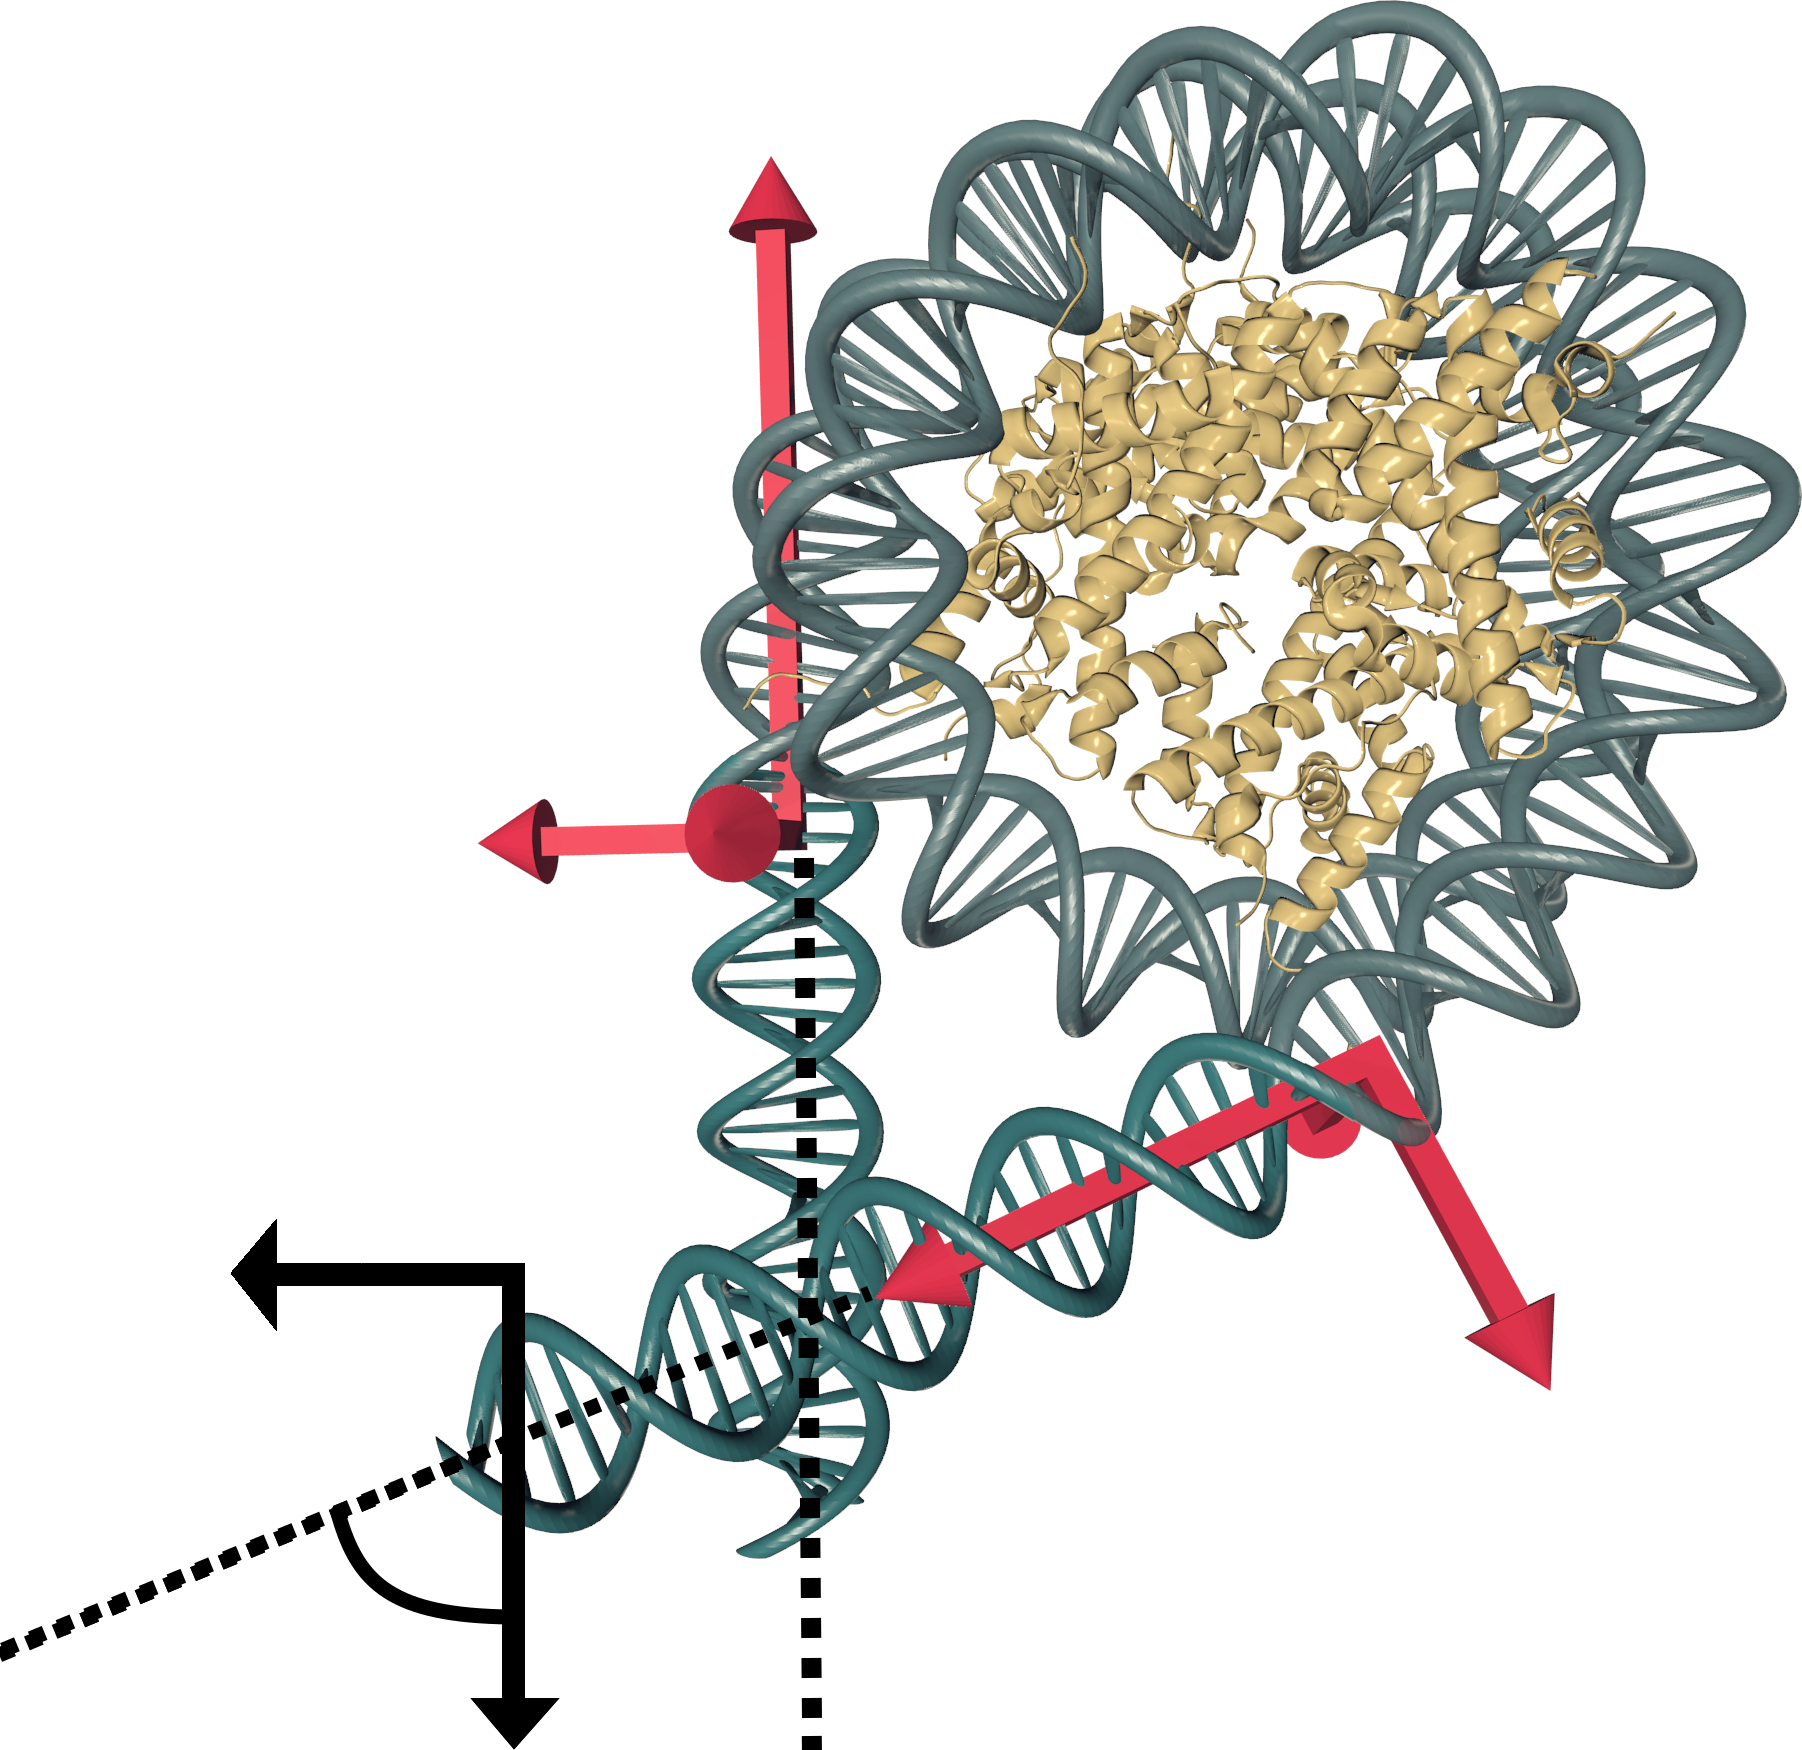
\includegraphics[width=0.35\linewidth]{./figures/fig-1a-nucleosome-geometry.png}
    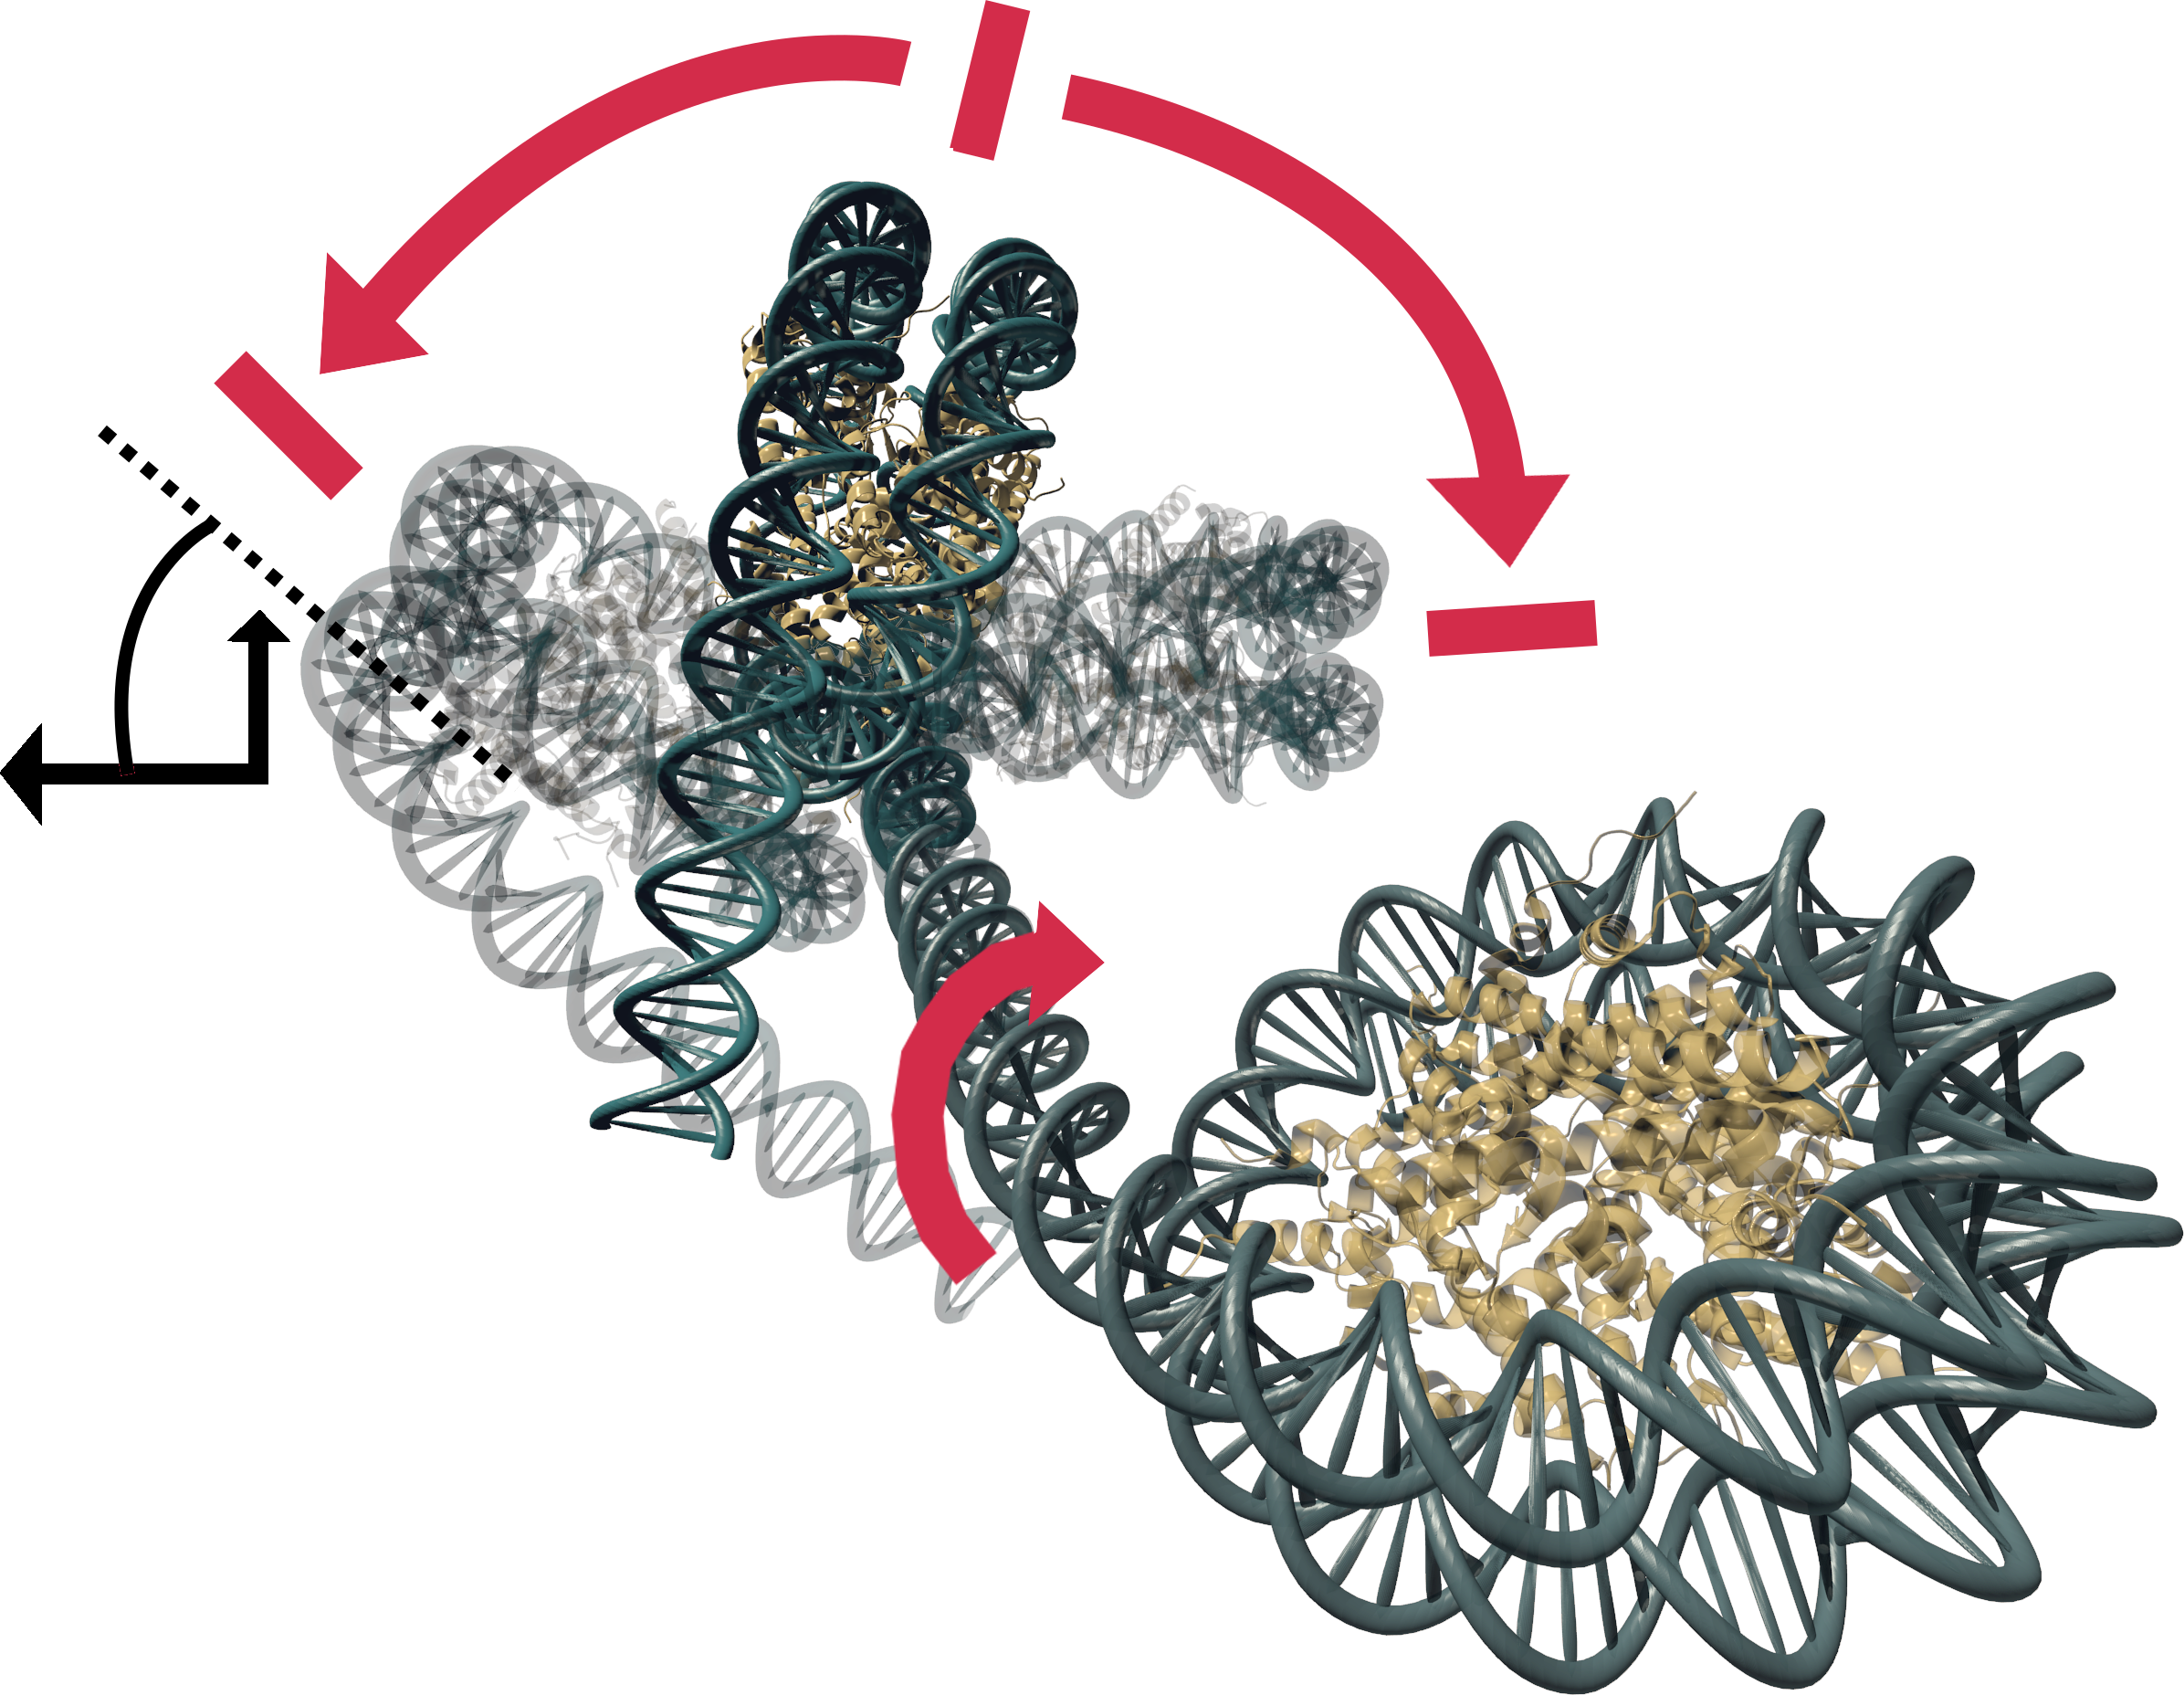
\includegraphics[width=0.52\linewidth]{./figures/fig-1b-helicity-effect.png}
    \caption{(a) When bound to a histone octamer, DNA traces out an
    approximately helical path. We treat the DNA bound to the histones as rigid,
    which corresponds to fixing the entry ($\Omega_\text{entry}$) and exit
    ($\Omega_\text{exit}$) orientations of the DNA from the nucleosome relative
    to each other ($\Omega_\text{nuc} =
    \Omega_\text{entry}^{-1}\Omega_\text{exit}$).
    (b) The DNA double helix has an intrinsic twist, $\tau$. At zero
    temperature, if we hold the location of one nucleosome constant, the binding
    orientation of the next histone octamer must change so that it aligns with
    the major groove of the double helix. This means that as the linker
    connecting two nucleosomes gets longer or shorter, their relative
    orientations with change by an angle proportional to $\tau$.}
\end{figure}

\section{Outline}
\begin{enumerate}
    \item introduction
    \begin{enumerate}
        \item dna is fundamental blueprint of life
        \item much of dna expression, as well as genetic inheritance, depends on the
            structure (and dynamics, see e.g.\ homolog recombination) of DNA.\
        \item nucleosome definition
    \end{enumerate}

    \item results
    \begin{enumerate}
        \item something
    \end{enumerate}

    \item discussion
    \begin{enumerate}
        \item something
    \end{enumerate}
\end{enumerate}


\begin{figure}[t]
    \centering
    \begin{minipage}{0.65\linewidth}
        \includegraphics[width=1\linewidth]{./figures/fig-2a-kuhn-all.png}
    \end{minipage}
    \begin{minipage}{0.30\linewidth}
        \vfill
        \includegraphics[width=1\linewidth]{./figures/fig-2b-mc-example.png}
        \vfill
    \end{minipage}
    \\
    \includegraphics[width=0.95\linewidth]{./figures/fig-2c-kuhn-zoom.png}
    \caption{(a) }
\end{figure}
\begin{figure}[t]
    \centering
    \includegraphics[width=0.95\linewidth]{./figures/fig-3-box-variance.png}
    \caption{A caption.}
\end{figure}
\begin{figure}[t]
    \centering
    \includegraphics[width=0.95\linewidth,height=0.6\linewidth]{./figures/fig-4-exp-variance.png}
    \caption{A caption.}
\end{figure}
\begin{figure}[t]
    \centering
    \includegraphics[width=0.55\linewidth]{./figures/fig-5a-exp-looping.png}
    \includegraphics[width=0.35\linewidth]{./figures/fig-5b-looping-features.png}
    \caption{A caption.}
\end{figure}

\section{PRL Guidelines}

Must be submitted to a section, closest fits seem to be:
L0-06: Statistical Physics and Thermodynamics
L3-30: Dynamics and Structure of Atoms and Molecules
L6-60: Chemical Physics
but espeically these two:
L8-81: Biological and Medical Physics
L8-78: Liquid Crystals and Polymers


3750 words

Include:

Any text in the body of the article;
Any text in a figure caption or table caption;
Any text in a footnote or an endnote

Exclude:

Title;
Author and affiliation listing;
Abstract;
Receipt date, published date, and other publication history;
PACS or Keywords and DOI;\@
References;
Author byline footnotes;
Acknowledgments

Estimating the word equivalent for figures can be simplified by using the aspect
ratio (width / height) of the figure. The estimates would be ((150 / aspect
ratio) + 20 words) for single-column figures, and ((300 / (0.5 * aspect ratio))
+ 40 words) for double column figures.

The word equivalent for displayed math is 16 words per row for single-column
equations. Two-column equations count as 32 words per row.

% \section{\label{sec:level1}First-level heading}

% This sample document demonstrates proper use of REV\TeX~4.1 (and
% \LaTeXe) in mansucripts prepared for submission to APS
% journals. Further information can be found in the REV\TeX~4.1
% documentation included in the distribution or available at
% \url{http://authors.aps.org/revtex4/}.

% When commands are referred to in this example file, they are always
% shown with their required arguments, using normal \TeX{} format. In
% this format, \verb+#1+, \verb+#2+, etc. stand for required
% author-supplied arguments to commands. For example, in
% \verb+\section{#1}+ the \verb+#1+ stands for the title text of the
% author's section heading, and in \verb+\title{#1}+ the \verb+#1+
% stands for the title text of the paper.

% Line breaks in section headings at all levels can be introduced using
% \textbackslash\textbackslash. A blank input line tells \TeX\ that the
% paragraph has ended. Note that top-level section headings are
% automatically uppercased. If a specific letter or word should appear in
% lowercase instead, you must escape it using \verb+\lowercase{#1}+ as
% in the word ``via'' above.

% \subsection{\label{sec:level2}Second-level heading: Formatting}

% This file may be formatted in either the \texttt{preprint} or
% \texttt{reprint} style. \texttt{reprint} format mimics final journal output.
% Either format may be used for submission purposes. \texttt{letter} sized paper should
% be used when submitting to APS journals.

% \subsubsection{Wide text (A level-3 head)}
% The \texttt{widetext} environment will make the text the width of the
% full page, as on page~\pageref{eq:wideeq}. (Note the use the
% \verb+\pageref{#1}+ command to refer to the page number.)
% \paragraph{Note (Fourth-level head is run in)}
% The width-changing commands only take effect in two-column formatting.
% There is no effect if text is in a single column.

% \subsection{\label{sec:citeref}Citations and References}
% A citation in text uses the command \verb+\cite{#1}+ or
% \verb+\onlinecite{#1}+ and refers to an entry in the bibliography.
% An entry in the bibliography is a reference to another document.

% \subsubsection{Citations}
% Because REV\TeX\ uses the \verb+natbib+ package of Patrick Daly,
% the entire repertoire of commands in that package are available for your document;
% see the \verb+natbib+ documentation for further details. Please note that
% REV\TeX\ requires version 8.31a or later of \verb+natbib+.

% \paragraph{Syntax}
% The argument of \verb+\cite+ may be a single \emph{key},
% or may consist of a comma-separated list of keys.
% The citation \emph{key} may contain
% letters, numbers, the dash (-) character, or the period (.) character.
% New with natbib 8.3 is an extension to the syntax that allows for
% a star (*) form and two optional arguments on the citation key itself.
% The syntax of the \verb+\cite+ command is thus (informally stated)
% \begin{quotation}\flushleft\leftskip1em
% \verb+\cite+ \verb+{+ \emph{key} \verb+}+, or\\
% \verb+\cite+ \verb+{+ \emph{optarg+key} \verb+}+, or\\
% \verb+\cite+ \verb+{+ \emph{optarg+key} \verb+,+ \emph{optarg+key}\ldots \verb+}+,
% \end{quotation}\noindent
% where \emph{optarg+key} signifies
% \begin{quotation}\flushleft\leftskip1em
% \emph{key}, or\\
% \texttt{*}\emph{key}, or\\
% \texttt{[}\emph{pre}\texttt{]}\emph{key}, or\\
% \texttt{[}\emph{pre}\texttt{]}\texttt{[}\emph{post}\texttt{]}\emph{key}, or even\\
% \texttt{*}\texttt{[}\emph{pre}\texttt{]}\texttt{[}\emph{post}\texttt{]}\emph{key}.
% \end{quotation}\noindent
% where \emph{pre} and \emph{post} is whatever text you wish to place
% at the beginning and end, respectively, of the bibliographic reference
% (see Ref.~[\onlinecite{witten2001}] and the two under Ref.~[\onlinecite{feyn54}]).
% (Keep in mind that no automatic space or punctuation is applied.)
% It is highly recommended that you put the entire \emph{pre} or \emph{post} portion
% within its own set of braces, for example:
% \verb+\cite+ \verb+{+ \texttt{[} \verb+{+\emph{text}\verb+}+\texttt{]}\emph{key}\verb+}+.
% The extra set of braces will keep \LaTeX\ out of trouble if your \emph{text} contains the comma (,) character.

% The star (*) modifier to the \emph{key} signifies that the reference is to be
% merged with the previous reference into a single bibliographic entry,
% a common idiom in APS and AIP articles (see below, Ref.~[\onlinecite{epr}]).
% When references are merged in this way, they are separated by a semicolon instead of
% the period (full stop) that would otherwise appear.

% \paragraph{Eliding repeated information}
% When a reference is merged, some of its fields may be elided: for example,
% when the author matches that of the previous reference, it is omitted.
% If both author and journal match, both are omitted.
% If the journal matches, but the author does not, the journal is replaced by \emph{ibid.},
% as exemplified by Ref.~[\onlinecite{epr}].
% These rules embody common editorial practice in APS and AIP journals and will only
% be in effect if the markup features of the APS and AIP Bib\TeX\ styles is employed.

% \paragraph{The options of the cite command itself}
% Please note that optional arguments to the \emph{key} change the reference in the bibliography,
% not the citation in the body of the document.
% For the latter, use the optional arguments of the \verb+\cite+ command itself:
% \verb+\cite+ \texttt{*}\allowbreak
% \texttt{[}\emph{pre-cite}\texttt{]}\allowbreak
% \texttt{[}\emph{post-cite}\texttt{]}\allowbreak
% \verb+{+\emph{key-list}\verb+}+.



\end{document}
